\section{Data}
% The data used for in-silico experiments are relative RNA expression levels describing how transcription levels are affected by different experimental conditions of gene manipulation, such as gene deletions (knockouts). Protein-protein interaction data is also used describing direct protein regulation, as well as protein-DNA interaction describing transcriptional control.


\subsection{DREAM challenge networks}
\begin{frame}<1-2>{DREAM challenge networks}
\label{sec:dream_data}
\begin{columns}
\begin{column}{0.4\textwidth}
% From DREAM challenge "DREAM4" 5 networks were available of 10 nodes each~(\autoref{fig:dream4_nets10}) as well as 5 networks of 100 nodes~(\autoref{fig:dream4_nets100})~\cite{dream4}. Networks with 10 nodes are referred to as 10.x and with 100 nodes named 100.x where x is in range~$[1,5]$.
DREAM4 simulated data~\cite{dream4}:
\begin{itemize}
    \item RNA expression at equilibrium for WT, single knockouts and knockdowns
    \item RNA expression at equilibrium for dual knockouts, and indexes of the knocked out genes
    \item time-series of RNA expression for single knockouts
    \item "gold standard" true edges
\end{itemize}
\end{column}

\begin{column}{0.6\textwidth}
\alt<1| handout:1>{
\begin{figure}[ht]
    \centering
    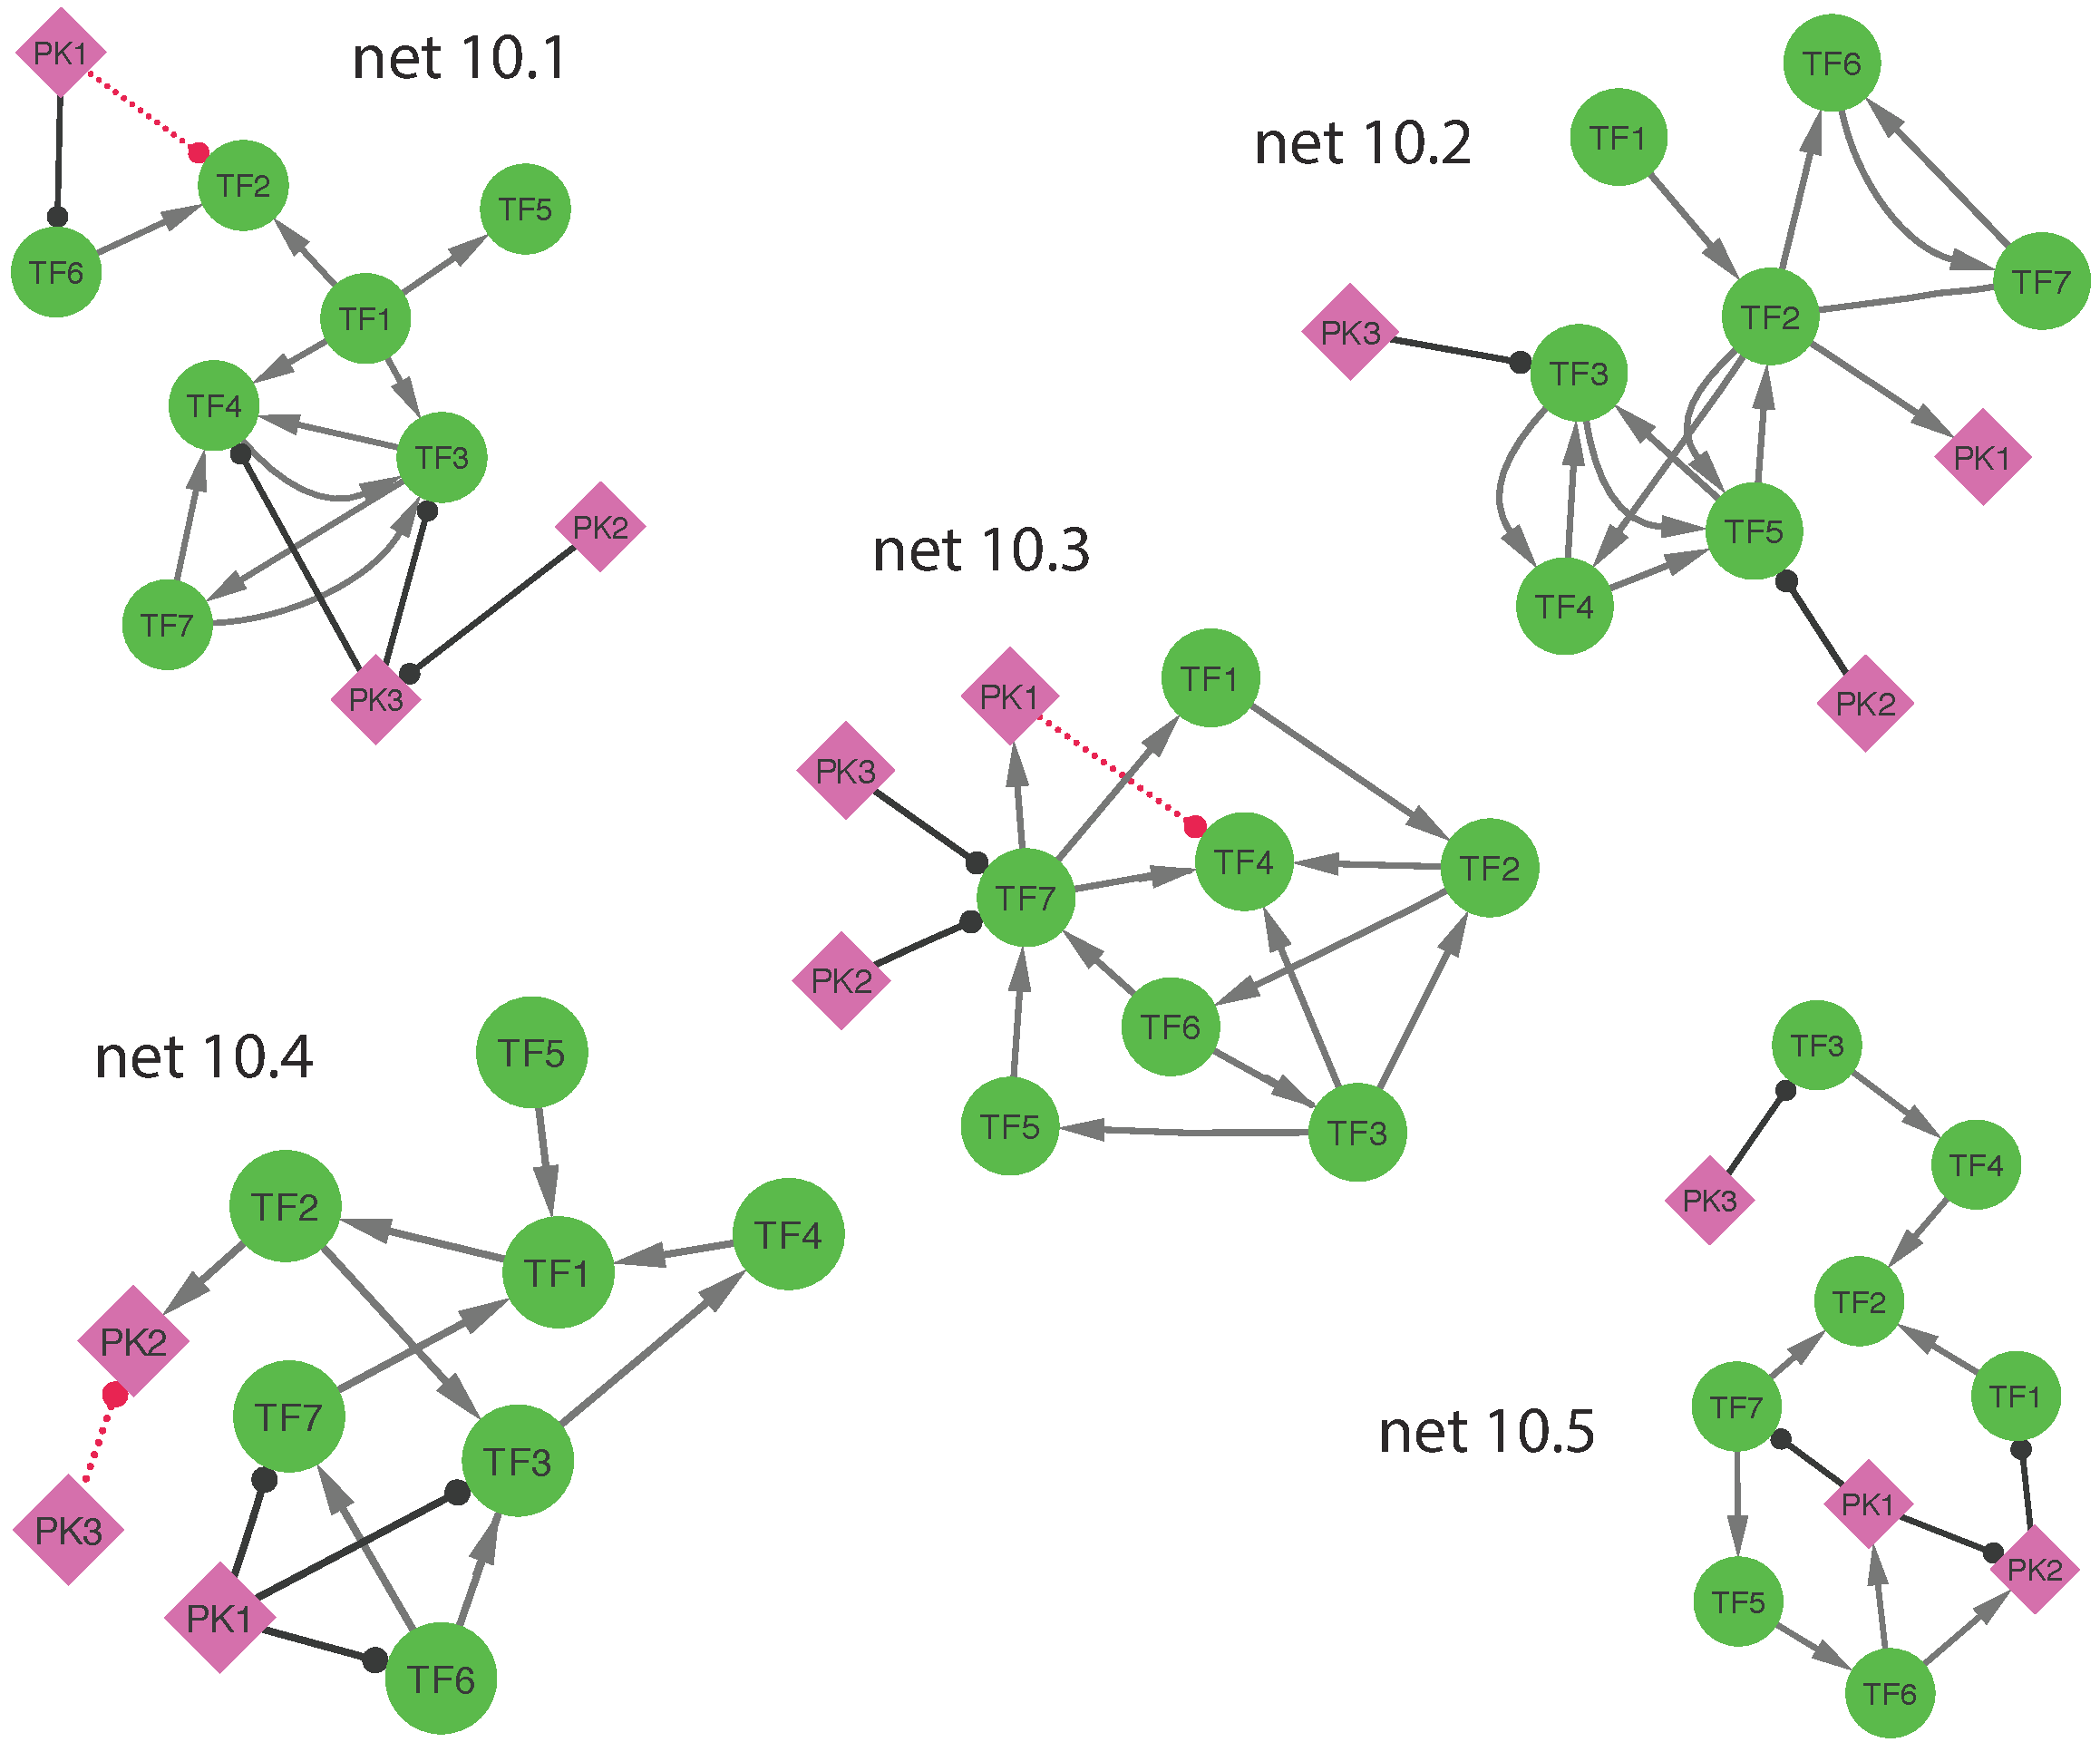
\includegraphics[height=0.85\textheight]{data/fig/nets_10.pdf}
    \caption{\textbf{Networks with 10 nodes.} \textcolor{gray}{Gray} = TF edge, \textcolor{black}{black} = detectable PK edge, \textcolor{red}{red} = silent PK edges. }
    \label{fig:dream4_nets10}
\end{figure}}
{\stepcounter{figure}
\begin{figure}[ht]
    \centering
    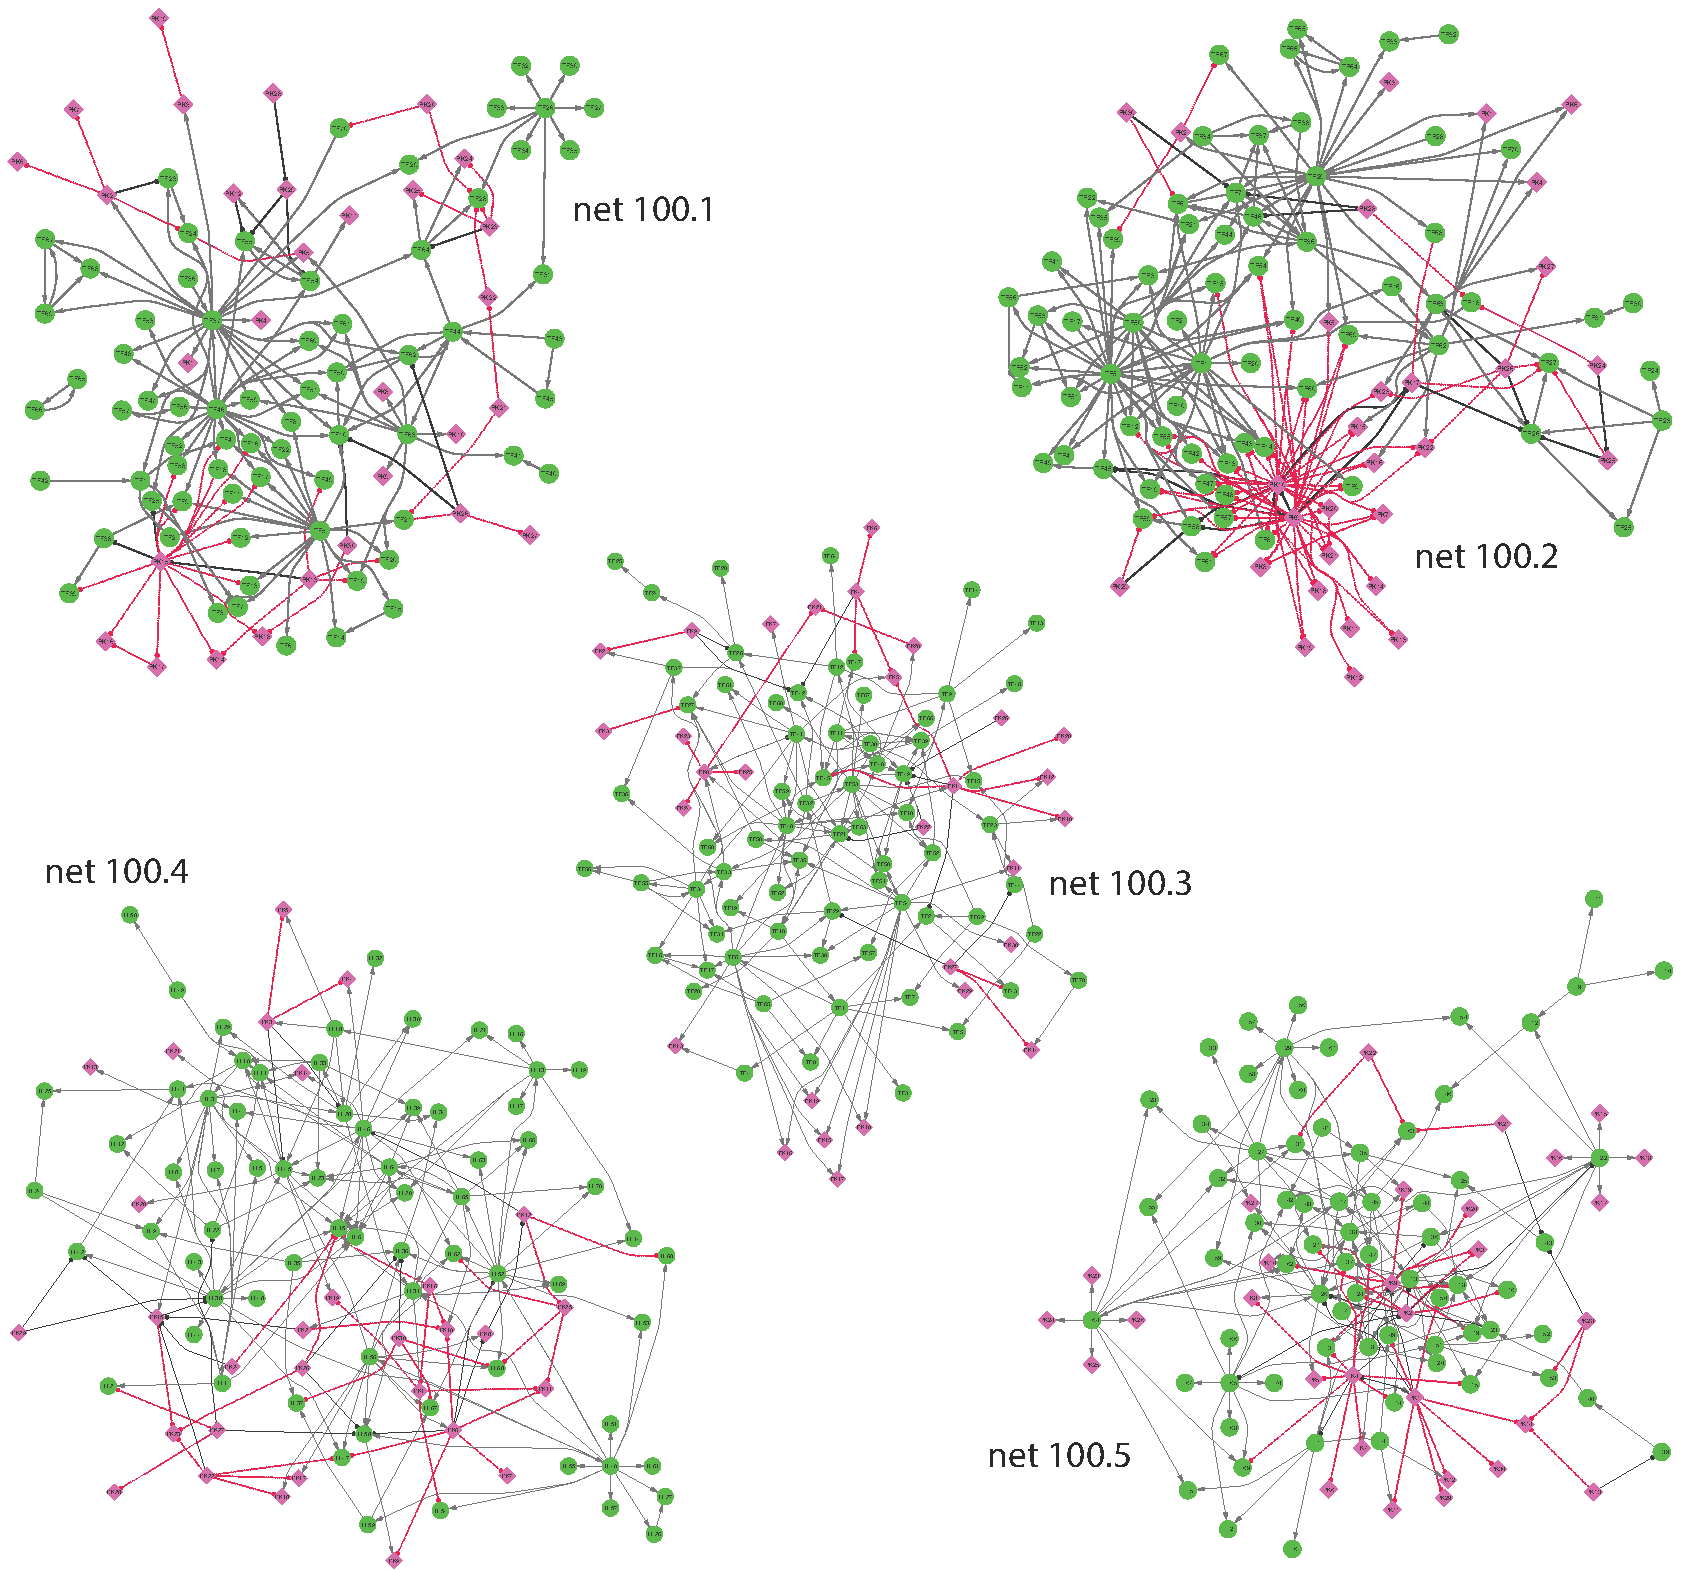
\includegraphics[height=0.85\textheight]{data/fig/nets_100.pdf}
    \caption{\textbf{Networks with 100 nodes.} \textcolor{gray}{Gray} = TF edge, \textcolor{black}{black} = detectable PK edge, \textcolor{red}{red} = silent PK edges. }
    \label{fig:dream4_nets100}
\end{figure}}
% The simulated RNA expression levels are not used since they are simulated using GeneNetWeaver which does not use kinase effects in its gene regulation model. The gold standard true edges are used here. They are given as a list of all pairs of nodes with a 1 or 0 to indicate presence or absence of a directed edge. This was formatted as an adjacency matrix of ones and zeros with edge source nodes as column names and edge target nodes as row names.
% The first~70\% of nodes are used as transcription factors and the remaining~30\% as kinase/phosphatases to roughly match the proportions observed in the yeast data~(\autoref{sec:yeast_data}). So, for 10 node networks there are 7 nodes assigned as TFs and 3 assigned as PKs, for 100 node networks there are 70 assigned as TFs and 30 as PKs.
% The graphs are shown for networks of 10 nodes~(\autoref{fig:dream4_nets10}), for networks of 100 nodes~(\autoref{fig:dream4_nets100}), as well as larger versions of 100 node networks~(\autoref{app:dream_nets}). Each graph are plotted with unsigned edges between TFs and PKs. As discussed in~\autoref{sec:unobservable}, there are certain circumstances where a PK to TF edge will be silent in RNA knockout measurements. These edges are here referred to as undetectable or silent edges.
\end{column}
\end{columns}
\end{frame}

% \begin{frame}{DREAM challenge networks}
% \begin{table}[ht]
% \caption{\textbf{Gold standard networks.} "detectable PK edge" = has effect on gene expression. "detectable PK nodes" = $\ge1$ detectable in- or outgoing edge. "nonsilent PK nodes" = $\ge1$ detectable outgoing edge. }
% \begin{tabularx}{\textwidth}{@{}XXXXXX@{}}
%     \toprule
%     & TF edges & PK edges & \pbox[t]{4cm}{detectable \\ PK edges} & \pbox[t]{4cm}{detectable \\ PK nodes} & \pbox[t]{4cm}{nonsilent \\ PK nodes} \\
%     \midrule
%     net 10.1 & 10 & 5 & 4 & 3 & 3 \\
%     net 10.2 & 14 & 2 & 2 & 3 & 2 \\
%     net 10.3 & 12 & 3 & 3 & 3 & 2 \\
%     net 10.4 & 9 & 4 & 3 & 2 & 1 \\
%     net 10.5 & 8 & 4 & 4 & 3 & 3 \\
%     net 100.1 & 176 & 48 & 13 & 19 & 9 \\
%     net 100.2 & 249 & 101 & 17 & 20 & 9 \\
%     net 100.3 & 195 & 28 & 11 & 23 & 7 \\
%     net 100.4 & 211 & 51 & 19 & 24 & 12 \\
%     net 100.5 & 193 & 52 & 15 & 23 & 7 \\
%     \bottomrule
% \end{tabularx}
% \label{tab:dream_data}
% \end{table}
% % Counts of nodes and edges are summarized in~\autoref{tab:dream_data}. Undetectable edges will not be considered for performance since they will not be detected regardless of inference method. This reduces the effective sizes of the graphs to having the number of PKs listed in column "detectable PK nodes" and to have the PK edges listed in "detectable PK edges".
% % To simulate node values, the gold standard edges are randomly signed and given a random strength. This is generally done by providing a random uniform number in range $[-1,1]$ for each nonzero entry in the gold standard adjacency matrix. It was also tested with standard Gaussian random values.
% % Gene expression levels as log fold-change RNA values are simulated using each of these networks for performance testing of edge inference. Simulation is performed using simple iteration discussed in~\autoref{sec:prim}, or using the GeneNetWeaver extension discussed in~\autoref{sec:gnw_extension}.
% \end{frame}

\begin{frame}{RNA expression levels}
\label{sec:yeast_data}
\begin{columns}
\begin{column}{0.3\textwidth}

% RNA expression levels are gathered from TF, kinase and phosphatase mutant experiments. The TF mutant experiment data were collected from Luscombe et al.~\cite{Luscombe2010} which is based on the original experiments by Hu~et~al.~\cite{Hu2007}. Luscombe et al. improved upon the statistical work performed by Hu~et~al. by considering things like multiple testing problems. The kinase and phosphatase mutant experiments are from Holstege~et~al.~\cite{Holstege2010}. The TF mutants are derived from a BY4741 strain and the kinase/phosphatase mutant from a BY4742 strain.
\small
TF: Luscombe~et~al.~\cite{Luscombe2010}, \\ originally Hu~et~al.~\cite{Hu2007} \\
PK: Holstege~et~al.~\cite{Holstege2010} \\
Name conversion: Tiger~et~al.~\cite{Tiger2012}
\normalsize
% The measurements are gathered for cells at mid log-phase mainly on rich media, but some experiments were done with heat-stress and other stresses. Log-phase is the phase in a typical growth curve of a microorganism where the cells are increasing in number exponentially. The measurements are taken at this time in an attempt to have the cells observed under uniform reproducible conditions with expression levels and regulation as constant as possible.
% The RNA concentrations are measured for both wildtype and the strain under the experimental conditions which in this case are different knockout background. For most experiments a single gene is knocked out, but for some kinase and phosphatase experiments multiple genes have been knocked out.
% The measurements provided are log fold-change values, which are log-transformed ratios comparing the RNA concentration in a knockout experiment with the wildtype concentration~(\autoref{eq:logFC}).

\begin{equation}
\label{eq:logFC}
    x_i = \log_2 \left( \frac{x_i^{(\text{ko})}}{x_i^{(\text{wt})}} \right)
\end{equation}
% Here $x_i$ is the provided transformed value. The superscripts $(\text{ko})$ and $(\text{wt})$ indicates RNA measurements for knockout and wildtype experiment, respectively.
% The values are provided in a table for TF knockouts and another for PK knockouts, each having the knocked out gene indicated as column names and the gene for which RNA is measured indicated as row names. The names are given as popular names, as opposed to systematic names~(ORF~names).
% The log fold-change values are distributed around zero as a bell-curve with lighter tails than a normal distribution~(\autoref{fig:RNA_hist}). The means are $\mu_T \approx -0.023$ and $\mu_P \approx 0.0030$, and standard deviations $\sigma_T \approx 0.24$ and $\sigma_P \approx 0.17$ for transcription factor and kinase/phosphatase knockout experiments, respectively. We see that the majority of genes are not affected strongly be any random knockout.
% From Luscombe~et~al. there are 269 experiments each with a single transcription factor knockout. From Holstege~et~al. there are 144 experiments with a single kinase or phosphatase knockout, 16 with double kinase or phosphatase knockout and a single experiment with a triple knockout totaling at 161 experiments. 5 experiments from Luscombe have the same gene knocked out as from Holstege. An overview of counts can be found in~\autoref{tab:process_counts}.
\end{column}

\begin{column}{0.7\textwidth}
\begin{figure}[ht]
  \centering
  \begin{subfigure}[t]{0.49\textwidth}
  \centering
  \caption{}
  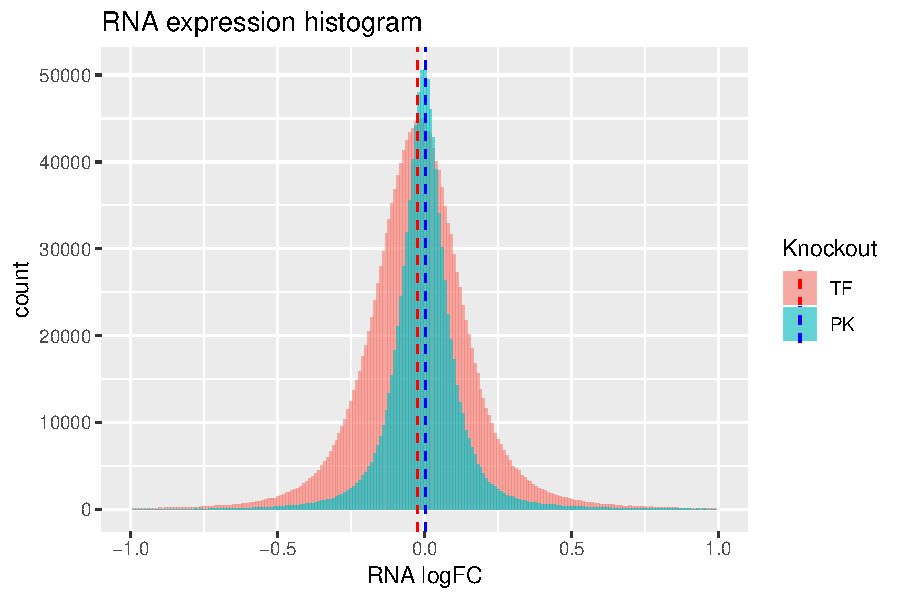
\includegraphics[width=\textwidth]{data/fig/RNA_hist.pdf}
  \label{fig:RNA_hist}
  \end{subfigure}
  \begin{subfigure}[t]{0.49\textwidth}
  \centering
  \caption{}
  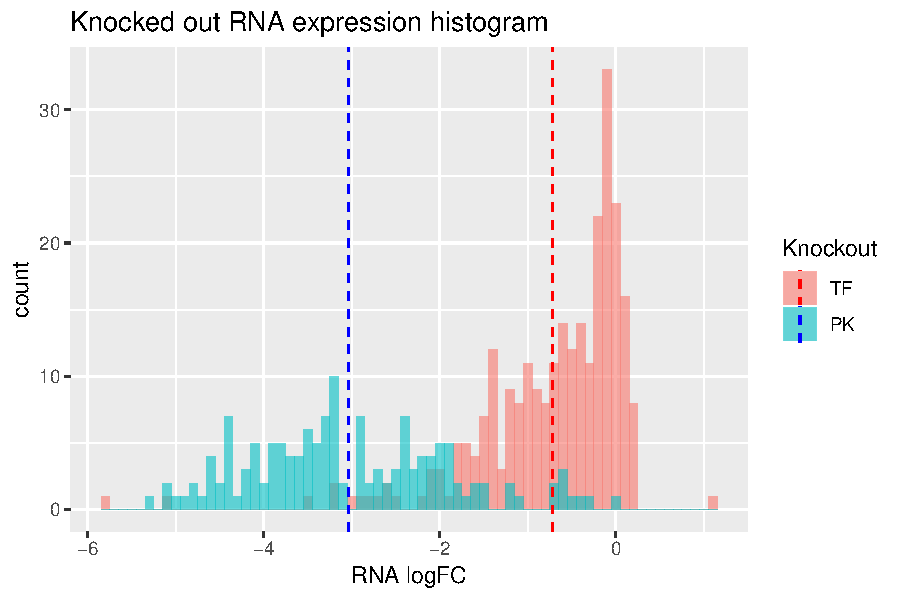
\includegraphics[width=\textwidth]{data/fig/knockout_RNA_hist.pdf}
  \label{fig:KO_RNA_hist}
  \end{subfigure}
  \caption{\textbf{RNA expression level histograms.} all (a) (TF: $269\cdot6253=\num{1.68e6}$, PK: $144\cdot6109=\num{0.88e6}$). Only KOs (b) (TF: 269, PK: 144). Dotted line = mean. }
\end{figure}
% Gene expression levels have been measured for all knockouts~(\autoref{fig:KO_RNA_hist}). The expression levels have mean $\mu_{T,KO} \approx -0.72$ and $\mu_{P,KO} \approx -3.0$ for transcription factor and kinase/phosphatase knockouts, respectively. As these are $\log_2$ fold-change values the means corresponds to a knocked out gene expressed ${\sim}1.6$ and ${\sim}8$ times less than wildtype for TF and PK, respectively.
\end{column}
\end{columns}
% Popular gene names were replaced with systematic names based on a conversion table from Tiger et al.~\cite{Tiger2012}.
% The simplest approach to format the data for use with the model is to filter it to enforce a perfect overlap in the genes for which log-fold change values are measured in the two datasets~(experiments with TF or PK knockouts). This makes it simple to concatenate measurements into a single matrix with known values at all entries.
% 
\small
\begin{table}[ht]
% \caption{\textbf{Protein types counted before and after preprocessing.} Counts of different types of proteins for which gene expression levels were measured. Counts are compared for raw data and data that has been filtered. TF KO, and PK KO refer to the work of Luscombe and Holstege, respectively. "PK and TF" refer to measurements of genes that are the intersection of the TF and PK sets and does therefore not add to the total. "neither" refers to genes that are never knocked out but still observed in the dataset. }
\begin{tabularx}{\textwidth}{@{}XXXXXX@{}}
    \toprule
    & TF & PK & PK and TF & neither & total \\
    \midrule
    TF KO & 269 & 144 & 5 & 5840 & 6253 \\
    PK KO & 266 & 144 & 5 & 5699 & 6109 \\
    processed & 266 & 144 & 5 & 5471 & 5881 \\
    \bottomrule
\end{tabularx}
\label{tab:process_counts}
\end{table}
\normalsize
% The filtering was performed, reducing the number of measured genes as described in \autoref{tab:process_counts}. Any measured gene is categorized as either a transcription factor, kinase/phosphatase, both or neither. We see that three TFs were not measured for kinase/phosphatase knockout experiments, which were removed both in terms of their knockout experiment as well as their expression level in knockout experiments of other transcription factors.

\end{frame}
\begin{frame}{Protein-promoter interactions}
% Data for proteins binding to promoters are gathered from Beyer and Workman et al.~\cite{BeyerWorkman2006}. It is a table of 13,239 transcription factor to gene interactions from 158 transcription factors, where each interaction has an assigned p-value.
Beyer and Workman et al.~\cite{BeyerWorkman2006}: 138 TFs (10,484 edges) \\
Yeastract~\cite{yeastract2017}: 173 TFs (136,813 edges)
\begin{figure}[ht]
  \centering
  \begin{subfigure}[t]{0.38\textwidth}
  \centering
  \caption{}
  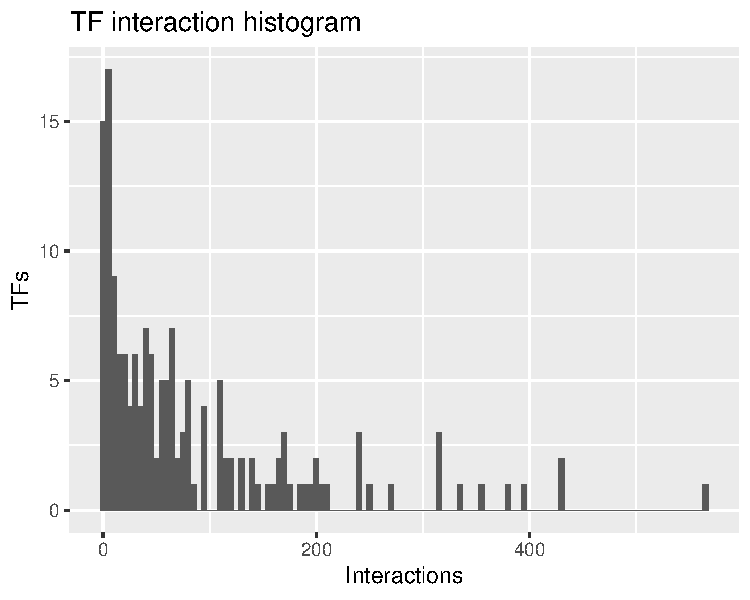
\includegraphics[width=\textwidth]{data/fig/TF_interaction_hist.pdf}
  \label{fig:TF_interactions_hist}
  \end{subfigure}
  \hfill
  \begin{subfigure}[t]{0.5\textwidth}
  \centering
  \caption{}
  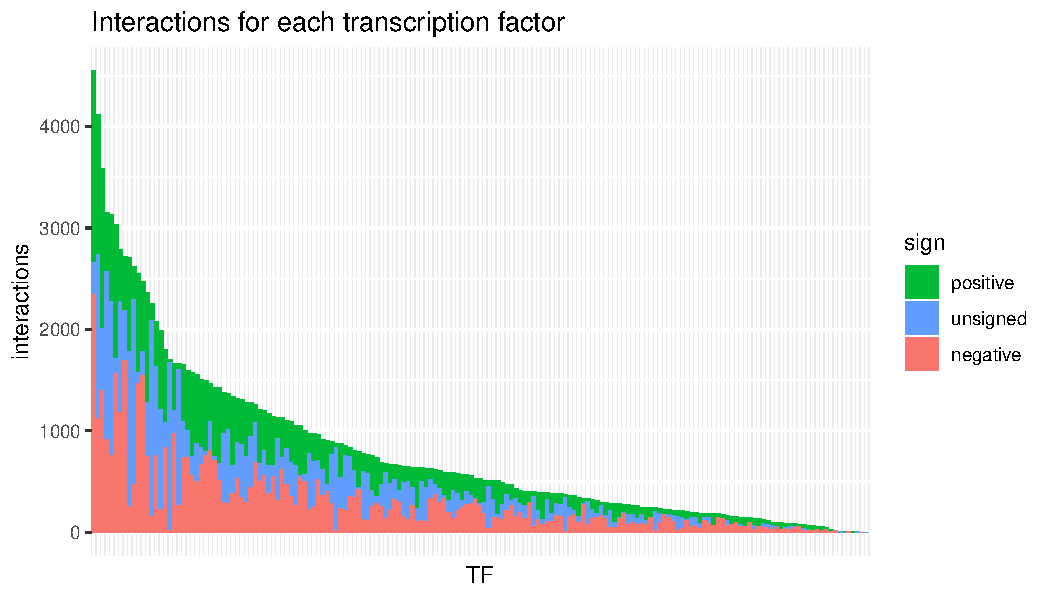
\includegraphics[width=\textwidth]{data/fig/yeastract.pdf}
  \label{fig:yeastract}
  \end{subfigure}
  \caption{\textbf{TF interactions.} TF$\rightarrow$gene interaction histogram for Beyer-Workman (a), and individual TF interactions for Yeastract (b). }
\end{figure}
% Most TFs in the data has in the range of ${\sim}10$ genes they are known to regulate but some regulate in the range of hundreds~(\autoref{fig:TF_interactions_hist}).
% The processed RNA values in \autoref{sec:yeast_data} have 5881 measurements for 266 TF knockout experiments, so not all knocked out TFs have known edges from this protein-promotor dataset. The overlap between the datasets reduces the number of edges from 13,239 to 10,484 with 128 of the 266 TFs having no known regulon. 
% The counts of different types of interactions for each of the 173 TFs are summarized in~\autoref{fig:yeastract}. Most TFs has more than 1 interaction and there is generally both activating and repressing interactions for any given TF. The TF with the most interactions is TF with ORF name YLR131C, which regulates 4550 unique genes in this dataset. 
\end{frame}

% \begin{frame}{Protein-promoter interactions - Yeastract}
% % Another dataset for transcription factors binding to DNA was found from Yeastract~\cite{yeastract2017}. The data was found by using the Yeastract website's function "Generate Regulation Matrix" retrieving all TF interactions documented with either DNA binding or expression evidence. The retrieval was performed separately for TFs acting as activator or inhibitor. The search was performed based on the systematic names of TFs and target genes from the TF dataset described in~\autoref{sec:yeast_data}, which is 266 TFs versus 5881 genes. The resulting tap-separated tables listing all regulatory interactions were used after having all the names converted to systematic names, since they are retrieved as popular names. The conversion was performed using Yeastract's own "ORF List to/from Gene List" conversion utility to ensure that all gene identifiers would be converted sucessfully back to ORF naming.
% % It is assumed that it is not known whether the protein-promotor interaction is positive or negative for TF-gene interactions that were listed in both the activator and repressor sets. They become defined here as unsigned edges, while the remaining activator and repressor interactions become defined as positive and negative edges. The counts of unique transcription factors found and TF-gene interactions are summarized in~\autoref{tab:yeastract}.
% \begin{table}[ht]
% \caption{\textbf{Yeastract TF interactions.} processed = assigning overlap in activators and inhibitors to a third "unsigned" category.}
% \begin{tabularx}{\textwidth}{@{}lYYYcYYYY@{}}
%     \toprule
%      & \multicolumn{3}{c}{raw} & \phantom{aa} & \multicolumn{4}{c}{processed} \\
%     \cmidrule{2-4} \cmidrule{6-9}
%      & activator & inhibitor & all && positive & negative & unsigned & all \\
%     \midrule
%     TFs & 170 & 173 & 173 && 167 & 171 & 157 & 173 \\
%     interactions & 85,098 & 94,286 & 179,384 && 42,527 & 51,715 & 42,571 & 136,813 \\
%     \bottomrule
% \end{tabularx}
% \label{tab:yeastract}
% \end{table}
% % The interactions were from 170 unique TFs in both the activator and repressor lists, as well as 3 additional unique TFs in the repressor list. After assigning the interactions a positive, negative, or unsigned edge, the counts of unique proteins remained about the same, indicating that a transcription factor will usually both have activating and repressing roles. There are $173 \cdot 5881 - 173 = 1,017,240$ possible edges from the TFs described in the Yeastract data to all of the measured genes, excluding self-interactions. About 13\% of possible edges are known~($136,813 / 1,017,240 \approx 0.134$), of which about 69\% have a known sign~($(42,527 + 51,715) / 136,813 \approx 0.689$).
% \end{frame}


% \begin{frame}{Protein-protein interactions}
\begin{columns}
\begin{column}{0.35\textwidth}
% Multiple datasets were found in an effort to have useful prior knowledge about known and probable PK$\rightarrow$PK and PK$\rightarrow$TF edges.

Fiedler~et~al.~\cite{Fiedler2009PK}
\label{sec:fiedler_data}

% Interaction data between proteins are gathered from Fiedler et al.~\cite{Fiedler2009PK}. The protein-protein interactions are from kinases and phosphatases interacting with other kinases, phosphatases and TFs. Fielder et al. collected a table of phosphorylation and dephosphorylation through manual curation of the literature. An Epistatic Miniarray Profile~(E-MAP) of 100,000 genetic interactions were then generated providing scored interactions.



% The scored data includes 537 interactions more for phosphate regulator partners that share a regulated substrate. 304 are pairs where each protein is a kinases or kinase regulator, 65 are pairs where each are phosphatases or phosphatase regulators, and 168 where it is a kinase and a phosphatase, or their regulator, sharing an interaction.

% All scored interactions are used as true interactions which is a total of $166 + 37 + 40 + 9 = 252$ scored interactions and $536 + 113 = 649$ unscored.

% The scored proteins and interactions are not distinct from the unscored ones. There are 63 unique proteins overlapping between scored and unscored datasets, and 206 unique interactions overlapping.


Yeast~KID~\cite{yeastkid}
\label{sec:yeastkid}

% 517 high confidence protein kinase interactions were collected from Yeast KID~\cite{yeastkid}. The table of interactions was found on \url{http://www.moseslab.csb.utoronto.ca/KID/} by searching for all interactions with p-value below 0.05 which is indicated on the page to correspond to a score above 4.52. The table can also be found as supplementary material to the publication which is without p-value cutoff. 74 of the PKs in the Yeast KID dataset overlap with the PKs in the knockout dataset~(\autoref{sec:yeast_data}).


Fasolo~et~al.~\cite{Fasolo2011}
\label{sec:fasolo}

% 1031 directed protein kinase interactions from 84 protein kinases were collected from the work of Fasolo~et~al.~\cite{Fasolo2011}. The proteins were given with popular and standard naming and was converted to systematic names using the conversion table from Tiger~et~al.~\cite{Tiger2012} as well as nomenclature obtained from the Saccharomyces Genome Database~\cite{yeastgenome}.
Name conversion: Tiger~et~al.~\cite{Tiger2012} and Saccharomyces Genome Database~\cite{yeastgenome}

BioGRID~\cite{BioGRID}

% Potential protein kinase interactions were collected from BioGRID~\cite{BioGRID}. Interactions were found from BioGRID's download page for latest release of kinome project interactions (\url{https://downloads.thebiogrid.org/BioGRID/Latest-Release/}). The table has a column describing if the interaction is physical or genetic, which was used to remove genetic interactions. The interactions does not have a described direction so all interactions were copied, reversed, reduced to unique interactions and then filtered so the source of each interaction is a protein kinase. This means that the interactions could be present but that it might be directed incorrectly so the dataset will be used for contrasting the other datasets where edges identified are assumed to be significantly more correct. By only using the 144 protein kinases that are knocked out in~\autoref{sec:yeast_data}, we get 1321 interactions. 
\end{column}

\begin{column}{0.65\textwidth}
\begin{table}[ht]
\caption{\textbf{(Un)scored (de)phosphorylations.} Fiedler et al. "direct" = protein performs (de)phosphorylation, "regulation" = protein regulates (de)phosphorylation through other kinase. Scored and unscored are not distinct. }
\begin{tabularx}{\textwidth}{@{}RYYcYY@{}}
    \toprule
     & \multicolumn{2}{c}{phosphorylation} & \phantom{aa} & \multicolumn{2}{c}{dephosphorylation} \\
    \cmidrule{2-3} \cmidrule{5-6}
     & direct & regulation && direct & regulation \\
    \midrule
    \textit{unscored}\phantom{...........} \\
    proteins & 79 & 34 && 26 & 9 \\
    interactions & 536 & 130 && 113 & 43 \\
    \textit{scored}\phantom{...............} \\
    proteins & 46 & 20 && 17 & 4 \\
    interactions & 166 & 37 && 40 & 9 \\
    \bottomrule
\end{tabularx}
\end{table}
\end{column}
\end{columns}
\end{frame}



\begin{frame}{Preprocessing}
\label{sec:data_preprocess}
\begin{columns}
\begin{column}{0.5\textwidth}

% All protein-DNA interactions were used as TF edges by matching the source of interaction against the 266 TF knocked out in experiments and the target against the 5881 measured genes. The result is a masking matrix, such that

Constrain to known TF edges
\begin{equation}     W^* = W \odot M
\end{equation}

% where $\odot$ is the Hadamard product~(element-wise), and masking matrix $M$ contains ones and zeros, with ones for each known TF interaction, for any PK to PK edges, and PK to TF edges. $W^*$ is the masked version of $W$ from~\autoref{eq:basic_eberhardt_extension}. $W$ holds the parameters that will be optimized in minimization of $\boldsymbol{e}$. A second matrix $S$ is created to control the signs of TF$\rightarrow$gene interactions. The matrix holds 1s for known positive interaction, -1s for known negative interactions and 0s for the remaining entries with the counts of positives and negatives described in~\autoref{tab:yeastract}. A new weight matrix where signs are controlled is then calculated as
Constraints on TF sign
\begin{subequations}
\begin{align}
W^{**} &= W^* \odot S^{(0)} + |W^*| \odot S
\\
s^{(0)}_{ij} &=
\begin{cases}
  1,
  & \text{if}\ s_{ij} = 0 \\
  0,
  & \text{otherwise}
\end{cases}
\end{align}
\end{subequations}
% Where $W^{**}$ is the new weight matrix used in place of $W$ in~\autoref{eq:basic_eberhardt_extension}, and $|W^*|$ indicates element-wise absolute values of $W^*$. Entries of $S_0$ is 1 if the equivalent entry in $S$ is zero, and 0 otherwise.
\end{column}
\begin{column}{0.5\textwidth}
Limit PK edges to edges from PK KOs onto PK/TF KOs
\begin{table}[ht]
\caption{\textbf{PK edges matching KOs.} Separated for high and low quality datasets. }
\begin{tabularx}{\textwidth}{@{}rYYY@{}}
    \toprule
     & \pbox{5em}{Fielder+Fasalo\\+YeastKID} & BioGRID & possible \\
    \midrule
    PK$\rightarrow$TF & 231 & 642 & 38,304 \\
    PK$\rightarrow$PK & 339 & 718 & 20,592 \\
    sum & 570 & 1360 & 58,896 \\
    \bottomrule
\end{tabularx}
\end{table}
\footnotesize
Fiedler~et~al.~\cite{Fiedler2009PK}
\label{sec:fiedler_data}
Yeast~KID~\cite{yeastkid}
\label{sec:yeastkid}
Fasolo~et~al.~\cite{Fasolo2011}
\label{sec:fasolo}
BioGRID~\cite{BioGRID}
Name conversion: Tiger~et~al.~\cite{Tiger2012} and Saccharomyces Genome Database~\cite{yeastgenome}
\normalsize
\end{column}
\end{columns}
\end{frame}

